% FILE: sentiment_lexica.tex  Version 0.01
% AUTHOR: Uladzimir Sidarenka

% This is a modified version of the file main.tex developed by the
% University Duisburg-Essen, Duisburg, AG Prof. Dr. Günter Törner
% Verena Gondek, Andy Braune, Henning Kerstan Fachbereich Mathematik
% Lotharstr. 65., 47057 Duisburg entstanden im Rahmen des
% DFG-Projektes DissOnlineTutor in Zusammenarbeit mit der
% Humboldt-Universitaet zu Berlin AG Elektronisches Publizieren Joanna
% Rycko und der DNB - Deutsche Nationalbibliothek

\section{Sentiment Lexica}\label{sec:snt:lex}

The first avenue that we are going to explore with the help of the
obtained corpus data is an automatic prediction of polar terms.
% To this end, we will first present an updated version of our dataset
% in Subsection~\ref{subsec:snt-lex:data} in which our experts revised
% the annotations of words and idioms that were present in the existing
% German sentiment lexica (GSL), but were not marked as emo-expressions
% in our data and, vice versa, were annotated as polar terms in the
% corpus, but absent in the analyzed polarity lists.
To this end, we will first evaluate the existing German sentiment
lexica (GSL) on our corpus data in order to obtain a baseline for the
subsequent experiments.  Since literally all of the current GSL were
created using an automatic translation of English opinion lists with a
manual post-editing of the translated entries, we will then look
whether the original methods that were used initially for creating the
English resources would yield better results when applied to German
data directly.  Finally, in the concluding step, we will analyze if
one of most popular areas of research in contemporary CL---distributed
vector representations of words \cite{Mikolov:13}---could be a more
perspective way for deriving new domain-specific polarity lists
without labeled data.  We will summarize and conclude in the last part
of this section, also discussing which of the presented methods
performed best on our corpus and explaining the reasons for this
success.

% \subsection{Data}\label{subsec:snt-lex:data}

% In the following experiments, we will use the updated version 0.1.0 of
% the sentiment dataset introduced in the previous section.  The main
% changes included in this version are:
% \begin{inparaenum}[\itshape a\upshape)]
%   \item the revision of the annotated emotional expressions, and
%   \item the addition of the boolean attributes \emph{subjective-fact}
%     and \emph{uncertain} to the annotation scheme of these elements.
% \end{inparaenum}

% To accomplish the fortmer objective, we compared the labelings of the
% opinionated terms in the first release of our corpus (version 0.0.1
% presented previously) with the entries from the existing German
% sentiment lexica: SentiWS \cite{Remus:10}, German Polarity Clues
% \cite{Waltinger:10}, and the Zurich Polarity List \cite{Clematide:10}.
% Similarly to the adjudication procedure used earlier, we automatically
% highlighted the differences between the corpus labels and the entries
% of these resources, letting our experts resolve the emerged conflicts.

% As it turned out, many of the contradicting cases stemmed from a
% different treatment of polar facts, such as ``Tod'' (\emph{death}),
% ``Anstieg'' (\emph{surge}), ``duften'' (\emph{to scent}) etc.: these
% entities were not labeled as emo-expressions in the full annotation of
% our dataset, but were still present as opinionated terms in the
% analyzed polarity lists.  Since these words represented a special
% class of polar clues due to their unequivocal objective nature, we
% decided to introduce a special feature called \emph{subjective-fact}
% into the attribute set of emotional expressions, explicitly asking our
% coders to annotate such terms with the emo-expression tag, but setting
% the value of the newly added attribute to \texttt{true}.

% The remaining differences were mainly due to polysemous words whose
% meaning in the corpus was not always subjective; errors in the lexica
% (GPC, for example, featured such auxiliary terms as ``sein'' (\emph{to
%   be}), ``wer'' (\emph{who}), or ``aus'' (\emph{from}) as opinionated
% entries); and, finally, numerous borderline cases which were difficult
% to resolve even in group discussions.  Examples of such challenging
% cases were words and idioms such as ``verbieten'' (\emph{to
%   prohibit}), ``verwechseln'' (\emph{to confuse}), ``Hauen und
% Stechen'' (\emph{hewing and stabbing}).  To address this issue, we
% again introduced an additional attribute, called \emph{uncertain},
% into the annotation scheme of emotional expressions and asked our
% experts to mark such borderline instances with this attribute.

% The statistics on the total number of the labeled elements and their
% agreement in the updated version are shown in
% Table~\ref{tbl:snt-lex:ucrp-agrmnt}:

% \begin{table*}[thb!]
%   \begin{center}
%     \bgroup \setlength\tabcolsep{0.7\tabcolsep} \scriptsize
%     \begin{tabular}{p{0.15\textwidth} % first columm
%         *{10}{>{\centering\arraybackslash}p{0.05\textwidth}}} % next ten columns
%       \toprule
%           \multirow{2}{0.2\textwidth}{\bfseries Element} &
%           \multicolumn{5}{c}{\bfseries Binary $\kappa$} & %
%           \multicolumn{5}{c}{\bfseries Proportional $\kappa$}\\
%           \cmidrule(r){2-6}\cmidrule(l){7-11}
%           & $M_1$ & $A_1$ & $M_2$ & $A_2$ & $\mathbf{\kappa}$ %
%           & $M_1$ & $A_1$ & $M_2$ & $A_2$ & $\mathbf{\kappa}$\\\midrule

%           EExpression &  &  &  & & \textbf{} & &  &  &  & \textbf{}\\
%           \bottomrule
%     \end{tabular}
%     \egroup
%   \end{center}
%   \captionof{table}{Inter-annotator agreement on the emotional
%     expression in the updated corpus.\\ {\small ($M1$ -- number of
%       tokens with matching labels in the first annotation, $A1$ --
%       total number of tokens labeled with that class in the first
%       annotation, $M2$ -- number of tokens with matching labels in the
%       second annotation, $A2$ -- total number of tokens labeled with
%       that class in the second annotation)}}
%   \label{tbl:snt-lex:ucrp-agrmnt}
% \end{table*}

\subsection{Evaluation of the Existing German Lexica}

In order to obtain a raw estimate of the expected scores for the
prediction of subjective expressions, we evaluated existing sentiment
lexica for German on the annotated data of our corpus.  The most
prominent of these resources are:
\begin{itemize}
\item the \textbf{German Polarity Clues} (GPC) list of
  \citet{Waltinger:10}, which comprises 10,141 subjective entries
  automatically translated from the English sentiment lexica
  \emph{Subjectivity Clues} \cite{Wilson:05} and \emph{SentiSpin}
  \cite{Takamura:05} with a subsequent manual rechecking of these
  translations and several synonyms and negated terms added by the
  authors;

\item the \textbf{SentiWS} (SWS) lexicon introduced by
  \citet{Remus:10}, which includes 1,818 positively and 1,650
  negatively connotated terms, also providing their part-of-speech
  tags and inflections (resulting in a total of 32,734 word forms).
  Similarly to the GPC, the authors used an English sentiment
  resource---the \emph{General Inquirer} list of \citet{Stone:66}---
  to bootstrap the entries for their lexicon, manually revising these
  automatic translations afterwards.  In addition to that,
  \citet{Remus:10} also expanded their polarity set with words and
  phrases frequently co-occurring with positive and negative seed
  lexemes using collocation information obtained from a corpus of
  10,200 customer reviews or extracted from the German Collocation
  Dictionary \cite{Quasthoff:10};

\item and, finally, the \textbf{Zurich Polarity List} developed by
  \citet{Clematide:10}, which comprises 8,000 subjective entries taken
  from GermaNet synsets \cite{Hamp:97}.  These synsets were manually
  annotated with their prior polarities by human experts.  Since the
  authors, however, found the number of polar adjectives obtained that
  way insufficient for running further classification experiments,
  they automatically enriched their lexicon with more attributive
  terms by analyzing conjoined collocations from a corpus using the
  method of \citet{Hatzivassi:97}.
\end{itemize}

In order to evaluate these resources on our dataset, we represented
each of the above lexicons as a trie \cite[pp. 492--512]{Knuth:98}
with the lexicon entries corresponding to paths in the resulting graph
and the polarity class(es) of these entries stored at the respective
terminal leaf nodes.  We then applied the standard match operation by
simultaneously checking the trie against contiguous runs of both
original and lemmatized corpus tokens.  All lemmatizations were done
using the \texttt{TreeTagger} \cite{Schmid:95}, and the match
operation was made case-insensitive.  Furthermore, since all analyzed
lexica only included plain textual terms, we also ignored smileys
during this comparison, solely concentrating on common lexical terms.

In this way, we estimated the precision, recall, and $F1$-score of the
positive, negative, and neutral polarity classes\footnote{We
  considered a term as neutral if it was not featured in the lexicon
  as either positive or negative entry.} of each lexicon by separately
computing these figures on each corpus file (99--109 tweets) and then
obtaining the mean and standard deviation of these scores over all
files in the dataset.  In addition to that, we also calculated the
macro- and micro-averaged results over all polarity classes.
Following the standard practice for computing these terms, we
estimated the macro-average as the mean of the $F1$-scores over all
three types (positive, negative, and neutral) and obtained the
micro-average by taking the harmonic mean of precision and recall
calculated over all true positives, false positives, and false
negatives found in the corpus.  The results of these computations are
shown in Table~\ref{snt-lex:tbl:gsl-res}.\footnote{For the sake of
  these experiments, we excluded the auxiliary words ``aus''
  (\emph{from}), ``der'' (\emph{the}), ``keine'' (\emph{no}),
  ``nicht'' (\emph{not}), ``sein'' (\emph{to be}), ``was''
  (\emph{what}), and ``wer'' (\emph{who}) with their inflection forms
  from the German Polarity Clues lexicon, since these entries
  significantly worsened the evaluation results.}

\begin{table}[h]
  \begin{center}
    \bgroup \setlength\tabcolsep{0.1\tabcolsep}\scriptsize
    \begin{tabular}{p{0.162\columnwidth} % first columm
        *{9}{>{\centering\arraybackslash}p{0.074\columnwidth}} % next nine columns
        *{2}{>{\centering\arraybackslash}p{0.068\columnwidth}}} % last two columns
      \toprule
          \multirow{2}*{\bfseries Lexicon} & %
          \multicolumn{3}{c}{\bfseries Positive Expressions} & %
          \multicolumn{3}{c}{\bfseries Negative Expressions} & %
          \multicolumn{3}{c}{\bfseries Neutral Terms} & %
          \multirow{2}{0.068\columnwidth}{\bfseries\centering Macro\newline $F1$} & %
          \multirow{2}{0.068\columnwidth}{\bfseries\centering Micro\newline $F1$}\\
          \cmidrule(lr){2-4}\cmidrule(lr){5-7}\cmidrule(lr){8-10}

          & Precision & Recall & $F1$ & %
          Precision & Recall & $F1$ & %
          Precision & Recall & $F1$ & & \\\midrule
      %% \multicolumn{9}{|c|}{\cellcolor{cellcolor}Existing Lexica}\\\hline

      GPC & 24\stddev{7.9} & 46.4\stddev{11.2} & 31.1\stddev{8.2} & %
      22\stddev{8.1} & 41.6\stddev{10.6} & 28.1\stddev{8.3} & %
      98\stddev{0.5} & 94.3\stddev{1} & 96.1\stddev{0.5} & %
      51.8\stddev{4.7} & 92.3\stddev{0.9}\\

      SWS & 35.9\stddev{13.2} & 38.7\stddev{11.6} & 36\stddev{9.9} & %
      49\stddev{17.1} & 31.3\stddev{10.9} & \textbf{37.2}\stddev{11.6} & %
      97.5\stddev{0.5} & 97.8\stddev{1} & 97.7\stddev{0.5} & %
      \textbf{56.9}\stddev{6.2} & 95.4\stddev{0.9}\\

      ZPL & 36.4\stddev{12.3} & 21.3\stddev{7.2} & 26.3\stddev{8} & %
      41.1\stddev{15.6} & 23.3\stddev{8.7} & 29\stddev{10} & %
      97\stddev{0.6} & 98.7\stddev{0.3} & 97.8\stddev{0.3} & %
      51.1\stddev{4.4} & 95.7\stddev{0.6}\\

      GPC $\cap$ SWS $\cap$ ZPL & \textbf{54}\stddev{12.8} & %
      30.6\stddev{10.5} & \textbf{38.1}\stddev{10.1} & %

      \textbf{61.7}\stddev{17.8} & 21.6\stddev{9.1} & 31.2\stddev{11.3} & %
      97.1\stddev{0.6} & \textbf{99.3}\stddev{0.3} & \textbf{98.2}\stddev{0.3} & %
      55.8\stddev{5.4} & \textbf{96.4}\stddev{0.6}\\

      GPC $\cup$ SWS $\cup$ ZPL & 23.3\stddev{7.6} & \textbf{48.5}\stddev{11.2} & %
      30.9\stddev{8.2} & %

      22\stddev{8} & \textbf{46.1}\stddev{10.8} & 29.1\stddev{8.5} & %
      \textbf{98.1}\stddev{0.5} & 93.9\stddev{1} & 96\stddev{0.5} & %
      52\stddev{4.8} & 92\stddev{0.9}\\\bottomrule
    \end{tabular}
    \egroup
    \caption{Evaluation of the existing German sentiment lexica.\\
      {\small (GPC -- German Polarity Clues \cite{Waltinger:10}, SWS
        -- SentiWS \cite{Remus:10}, ZPL -- Zurich Polarity Lexicon
        \cite{Clematide:10})}}
    \label{snt-lex:tbl:gsl-res}
  \end{center}
\end{table}

As can be seen from the table, the intersection of all three lexica
attains the best results on both positive and neutral classes, also
yielding the best scores in terms of the micro-averaged $F$-measure.
One of the main reasons for this success is a relatively high
precision of this list for all but the neutral polarity class, where
it is outperformed by the union of the three resources.  Not
surpisingly, the union also shows the highest recall of positive and
negative terms among all compared polarity lists.

Regarding the figures attained by the individual lexica, the best
results here are achieved by the SentiWS resource \cite{Remus:10},
which not only shows the highest $F1$-score for the negative terms but
also achieves the best macro-averaged $F1$-result on all classes.

At the same time, we also can observe that the deviation of the scores
on different files is relatively high.  In order to see whether this
skewness of the distribution could significantly affect the net
statistics, we additionally recomputed all results on the whole corpus
at once.  The updated figures are shown in
Table~\ref{snt-lex:tbl:gsl-res-full}.

\begin{table}[h]
  \begin{center}
    \bgroup \setlength\tabcolsep{0.1\tabcolsep}\scriptsize
    \begin{tabular}{p{0.162\columnwidth} % first columm
        *{9}{>{\centering\arraybackslash}p{0.074\columnwidth}} % next nine columns
        *{2}{>{\centering\arraybackslash}p{0.068\columnwidth}}} % last two columns
      \toprule
          \multirow{2}*{\bfseries Lexicon} & %
          \multicolumn{3}{c}{\bfseries Positive Expressions} & %
          \multicolumn{3}{c}{\bfseries Negative Expressions} & %
          \multicolumn{3}{c}{\bfseries Neutral Terms} & %
          \multirow{2}{0.068\columnwidth}{\bfseries\centering Macro\newline $F1$} & %
          \multirow{2}{0.068\columnwidth}{\bfseries\centering Micro\newline $F1$}\\
          \cmidrule(lr){2-4}\cmidrule(lr){5-7}\cmidrule(lr){8-10}

          & Precision & Recall & $F1$ & %
          Precision & Recall & $F1$ & %
          Precision & Recall & $F1$ & & \\\midrule
      %% \multicolumn{9}{|c|}{\cellcolor{cellcolor}Existing Lexica}\\\hline

      GPC & 23.83 & 46.8 & 31.58 & %
       22.37 & 41.58 & 29 & %
       98.01 & 94.27 & 96.1 & %
       52.26 & 91.32\\

      SWS & 34.36 & 39.23 & 36.63 & %
       49.56 & 31.45 & \textbf{38.48} & %
       97.5 & 97.84 & 97.67 & %
       \textbf{57.59} & 95.38\\

      ZPL & 36.4 & 21.22 & 26.81 & %
       41.57 & 23.14 & 29.73 & %
       96.96 & 98.73 & 97.84 & %
       51.46 & 95.67\\

      GPC $\cap$ SWS $\cap$ ZPL & \textbf{54.52} & 30.74 & \textbf{39.31} & %
       \textbf{62.92} & 21.68 & 32.25 & %
       97.13 & \textbf{99.25} & \textbf{98.18} & %
       56.58 & \textbf{96.39}\\

      GPC $\cup$ SWS $\cup$ ZPL & 23.11 & \textbf{48.86} & 31.38 & %
       22.42 & \textbf{46.05} & 30.16 & %
       \textbf{98.14} & 93.87 & 95.96 & %
       52.5 & 91.99\\\bottomrule
    \end{tabular}
    \egroup
    \caption{Evaluation of the existing German sentiment lexica on the
      complete corpus.\\ {\small (GPC -- German Polarity Clues
        \cite{Waltinger:10}, SWS -- SentiWS \cite{Remus:10}, ZPL --
        Zurich Polarity Lexicon \cite{Clematide:10})}}
    \label{snt-lex:tbl:gsl-res-full}
  \end{center}
\end{table}

As we can see from the scores, the relative placement of the
best-performing systems is the same as in the previous evaluation.
Moreover, the absolute results are only minimally higher (by typically
at most one percent) than the mean values computed in the previous
step.  Thus, even despite their high variance, the average figures
computed over single corpus files are still a reliable indicator of
the quality of the recognized opinionated terms.  For the sake of
brevity, we will therefore only present the former metric (the mean
and standard deviation of the scores estimated over individual files),
refraining from computing the statistics on the whole corpus in total.

\subsection{Evaluation of Dictionary-Based Lexicon Generation Approaches}

Since all of the presented works rely on a manual correction or
partial annotation of the lexicon entries, they clearly fall into the
category of semi-automatic approaches.  Unlike fully automated
methods, such systems typically yield more precise results, which,
however, come at the cost of tedious human efforts.  In order to see
to which extent these efforts really pay off in practice for the
lexicon generation (LG) task at hand, we additionally decided to
evaluate the most popular fully automatic LG approaches.

According to \citet[p. 79]{Liu:12}, most of such automated methods can
be divided into dictionary- and corpus-based ones.  The former
approaches try to derive polarity lists using monolingual thesauri or
lexical databases such as the Macquarie Dictionary \cite{Bernard:86}
or \textsc{WordNet} \cite{Miller:95}.  A clear advantage of these
systems is their relatively good precision as they operate on
carefully verified data enriched with hand-crafted meta information.
At the same time, this verification can become a drawback for the
recall in the domains where the language changes occur very rapidly,
and new terms are being coined in a flash.

The presumably first such approach was proposed by \citet{Hu:04}.  In
their work on sentiment classification and summarization of cutomer
reviews, the authors determined semantic orientation of adjectives
(which were supposed to be the most relevant part of speech for mining
people's opinions) by taking a set of seed terms with known polarities
and propagating these values to the synonyms of these words that were
found in \textsc{WordNet} \cite{Miller:95}.  A similar procedure was
applied to antonymous relations with the polarity orientation being
reversed during the propagation.  This expansion continued until no
more adjective could be reached via the synonymy-antonymy links.
Unfortunately, no intrinsic evaluation of the resulting lexicon was
performed in this work---the authors only report their results on
recognizing subjective sentences and classifying their polarity, where
they attain average \F-scores of 0.667 and 0.842 respectively.

Later on, this approach was refined by \citet{Blair-Goldensohn:08},
who obtained polarity labels for new words by multiplying a score
vector $v$ containing polarity scores of the known seed terms (-1 for
the negative expressions and 1 for the positive terms) with the
adjacency matrix $A$ constructed from the \textsc{WordNet} synsets.
In these experiments, the value of the adjacency cell $a_{ij}$ in the
matrix $A$ was set to $\lambda=0.2$ if there was a synonymy link
between the synsets $i$ and $j$ and to $-\lambda$ if these synsets
were antonymous to each other.  By performing this multiplication
multiple times and setting the $v$ vector to the result of the
previous iteration, the authors ensured that the polarity scores were
being propagated transitively through the network, decaying by a
constant factor ($\lambda$) with the increasing path length from the
original seeds.  This method again was evaluated only
extrinsically---the authors tested their complete sentiment
summarization system, which used the sentiment scores for individual
words as features for a maximum-entropy classifier.

With various modifications, the core idea of propagating the polarity
classes through the semantic graph was adopted in almost all of the
following dictionary-based works: \citet{Kim:04,Kim:06}, for instance,
used a similar method to determine the polarity of adjectives and
verbs given a small seed set of terms with known orientations.  In
particular, the likelihood of a new word $w$ belonging to the class $c
\in \{\textrm{postive}, \textrm{negative}, \textrm{neutral}\}$ was
computed as:
\begin{equation*}
  P(c|w) = \argmax_{c}P(c)P(w|c) = \argmax_{c}P(c)\frac{\sum\limits_{i=1}^{n}count(syn_i, c)}{count(c)},
\end{equation*}
where $P(c)$ is the prior probability of the polar class estimated as
the number of words with the given orientation $c$ divided by the
total number of terms considered, $count(syn_i, c)$ stands for the
number of times a seed term from class $c$ appears in a synset of $w$,
and $count(c)$ means the total number of synsets containing a seed
item.

Starting from a seed set of 34 adjectives and 44 verbs, the authors
successively expanded their lexicon to a list of 18,192 terms and
evaluated it on a manually labeled collection of 462 adjectives and
502 verbs taken from the TOEFL test and analyzed by two human experts.
The reported average accuracy for this method run up to 68.48\% for
adjectives and 74.28\% for verbs with their recall being equal to
93.07\% and 83.27\% respectively.  It should, however, be noted that
\citet{Kim:04} used a lenient metric for their computation by
considering neutral and positive terms as the same class which could
significantly boost the results.

% An alternative way of bootstrapping polarities for adjectives was
% proposed by \citet{Kamps:04}.  The authors estimated the orientation
% of the given term by computing the difference between the shortest
% path lengths of this word to the prototypic positive and negative
% lexemes---``good'' and ``bad''.  For example, the polarity score of
% the adjective ``honest'' was calculated as
% \begin{equation*}
%   POL(honest) = \frac{d(\textrm{honest}, \textrm{bad}) - d(\textrm{honest}, \textrm{good})}%
%   {d(\textrm{bad}, \textrm{good})} = \frac{6 - 2}{4} = 1,
% \end{equation*}
% where $d(w_1, w_2)$ means the geodesic (shortest-path) distance
% between the words $w_1$ and $w_2$ in the \textsc{WordNet} graph.  The
% respective orientation of this term was then correspondingly set to
% \texttt{positive} according to the sign of the obtained
% $POL$-value. \citet{Kamps:04} evaluated the accuracy of their method
% on the General Inquirer lexicon \cite{Stone:66} by comparing the terms
% with non-zero scores to the entries from this resource, getting
% 68.19\% of correct predictions on a set of 349 adjectives.

One of the most popular dictionary-based approaches to date, however,
was proposed by \citet{Esuli:06c}.  Starting with the positive and
negative seed sets used by \citet{Turney:03} and considering the rest
of the terms as objective if these words neither appeared in the
aforemention seed lists nor had a subjective tag in the General
Inquirer lexicon \cite{Stone:66}, the authors successively expanded
these polar sets for $k \in \{0, 2, 4, 6\}$ iterations by following
the synonymity-antonymity links similarly to the method proposed by
\citet{Hu:04}.\footnote{More precisely, following the work of
  \citet{Strapparava:04}, the authors propagated the same polarity
  values via the relations \emph{similarity}, \emph{derived-from},
  \emph{pertains-to}, and \emph{also-see}, and changed these values to
  the opposite when spreading them over the \emph{direct-antonymy}
  links.}  In each of these steps, they trained two types of ternary
classifiers---Rocchio and SVM---using tfidf-vectors of the training
glosses (whose amount was different in each iteration) as input
features.  \citet{Esuli:06c} experimented with two different ways of
obtaining such ternary predictors: using a committee of binary
classifiers and by directly training a ternary classification system,
finding that the latter option produced slightly better scores.  This
time, the evaluation was run on both the intersection with the
GI~lexicon~\cite{Stone:66} and a manually annotated subset of
\textsc{WordNet} synsets, yielding 66\% accuracy for the former
metric.\footnote{Note that different publications on
  \textsc{SentiWordNet} report different configuration settings,
  cf. \citet{Esuli:05}, \citet{Esuli:06a}, \citet{Esuli:06b}, and
  \citet{Esuli:06c}.  In our experiments, we will rely on the setup
  described in last paper as the most recent description of this
  approach.}

Finally, \citet{Rao:09} proposed another graph-based approach in which
they tried three different methods of assigning polarity scores to the
\textsc{WordNet} synsets:
\begin{inparaenum}[\itshape a\upshape)]
\item deterministic min-cut \cite{Blum:01},
\item randomized min-cut \cite{Blum:04}, and
\item the label propagation algorithm of \citet{Zhu:02}.
\end{inparaenum}
An evaluation of these systems on the GI lexicon \cite{Stone:66}
showed significant improvement over the previous baselines
\cite{Kamps:04,Kim:06}, with the deterministic min-cut yielding an
average \F{}-score of 0.833 over the three main parts of speech
(nouns, adjectives, and verbs) and the label propagation algorithm
reaching remarkable 0.916 average \F{} on nouns and verbs.\footnote{In
  order to obtain such high results, the authors had to use the
  hypernymy relation in addition to the normal synonymy links.  Since
  this relation was missing for adjectives, the results for this part
  of speech were significantly lower, only amounting to 0.73 \F{}.}

Other notable works on dictionary-based lexicon generation include
those of \citet{Mohammad:09}, who generated their seed set using
antonymous morphological patterns (e.g.,
\emph{logical}---\emph{illogical}, \emph{honest}---\emph{dishonest},
\emph{happy}---\emph{unhappy}) and subsequently expanded these seed
sets with the help of the Macquarie Thesaurus \cite{Bernard:86};
\citet{Awadallah:10}, who adopted a random walk approach, estimating
the polarity of an unknown word by taking the difference between an
average number of steps a random walker had to make in order to reach
a term from positive or negative set; and \citet{Dragut:10}, who
deduced the polarities of new words using manually specified inference
rules.

Since almost all of the presented approaches used \textsc{WordNet}---a
large lexical database with more than 117,000 synsets---and evaluated
their results in vitro (using the General Inquirer lexicon
\cite{Stone:66}), it remains unclear how these methods would work for
languages with smaller lexical resources and whether they would
perform equally well in vivo (when tested on a real-life corpus).
Moreover, because General Inquirer is a generic standard-language
dictionary, it is also not obvious whether the systems that perform
best on this list would be also applicable to more colloquial domains.

To answer these questions, we decided to reimplement the approaches of
\citet{Hu:04}, \citet{Blair-Goldensohn:08}, \citet{Kim:04,Kim:06},
\citet{Esuli:06c}, \citet{Rao:09}, and \citet{Awadallah:10}, applying
these methods to \textsc{GermaNet}---the German equivalent of the
English \textsc{WordNet} \cite{Hamp:97}\footnote{Throughout our
  experiments, we will use \textsc{WordNet} Version 3.0 and
  \textsc{GermaNet} Version 9.}--- and subsequently evaluating their
results on our presented Twitter corpus.

In order to make this comparison more fair, we used the same set of
the initial seed terms for all tested methods.  For this purpose, we
translated the original list of 14 subjectively connotated English
adjectives suggested by \citet{Turney:03}---\emph{good}$^+$,
\emph{nice}$^+$, \emph{excellent}$^+$, \emph{positive}$^+$,
\emph{fortunate}$^+$, \emph{correct}$^+$, \emph{superior}$^+$,
\emph{bad}$^-$, \emph{nasty}$^-$, \emph{poor}$^-$,
\emph{negative}$^-$, \emph{unfortunate}$^-$, \emph{wrong}$^-$, and
\emph{inferior}$^-$---into German, getting a total of 20 seeds (10
positive and 10 negative adjectives) due to multiple possible
translations of the same words.\footnote{The reimplemented methods and
  translated seed sets used in these experiments are available online
  at \url{https://github.com/WladimirSidorenko/SentiLex}.}
Furthermore, to settle the differences between the binary and ternary
approaches (i.e., those approaches that only differentiate between the
positive and negative classes and those ones which also discern the
neutral terms as a separate group), we additionally enriched the
translated seed set with 10 purely objective adjectives---``neutral''
(\emph{neutral}), ``sachlich'' (\emph{objective}), ``technisch''
(\emph{technical}) ``chemisch'' (\emph{chemical}), ``physisch''
(\emph{physical}), ``materiell'' (\emph{material}), ``k\"orperlich''
(\emph{bodily}), ``finanziell'' (\emph{financial}), ``theoretisch''
(\emph{theoretical}), and ``praktisch'' (\emph{practical})---letting
all evaluated classifiers work in the ternary mode.  Finally, since
different methods relied on various notions of synonymous relations
(e.g., \citet{Hu:04} only considered two words as synonyms if they
appeared together in the same synset whereas \citet{Esuli:06c},
\citet{Rao:09}, and \citet{Awadallah:10} also considered
hyper-hyponymous connections as valid edges for propagating the
polarity of the seed terms), we decided to unify this aspect too,
letting all systems work with an extended set of links.  Into this
set, we not only included the traditional synonymity relations for the
terms co-occurring in the same synsets but also established edges
between words if their synsets were conected via the inter-synset
links \texttt{has\_participle}, \texttt{has\_pertainym},
\texttt{has\_hyponym}, \texttt{entails}, or \texttt{is\_entailed\_by}.
We intentionally excluded the relations \texttt{has\_hypernym} and
\texttt{is\_related\_to} from this set, since hypernyms were not
guaranteed to preserve the polarity of their children---e.g.,
``bewertungsspezifisch'' (\emph{appraisal-specific} is a neutral term
in contrast to its immediate hyponyms ``gut'' (\emph{good}) and
``schlecht'' (\emph{bad})---and the \texttt{is\_related\_to} links
could connect both synonymous and antonymous terms---e.g., this type
of relation holds between the words ``Form'' (\emph{shape}) and
``unf\"ormig'' (\emph{misshapen}).

The results of our re-implementations are shown in
Table~\ref{snt-lex:tbl:lex-res}.

\begin{table}[h]
  \begin{center}
    \bgroup \setlength\tabcolsep{0.1\tabcolsep}\scriptsize
    \begin{tabular}{p{0.1\columnwidth} % first columm
        *{9}{>{\centering\arraybackslash}p{0.084\columnwidth}} % next nine columns
        *{2}{>{\centering\arraybackslash}p{0.078\columnwidth}}} % last two columns
      \toprule
          \multirow{2}*{\bfseries Lexicon} & %
          \multicolumn{3}{c}{\bfseries Positive Expressions} & %
          \multicolumn{3}{c}{\bfseries Negative Expressions} & %
          \multicolumn{3}{c}{\bfseries Neutral Terms} & %
          \multirow{2}{0.068\columnwidth}{\bfseries\centering Macro\newline $F1$} & %
          \multirow{2}{0.068\columnwidth}{\bfseries\centering Micro\newline $F1$}\\
          \cmidrule(lr){2-4}\cmidrule(lr){5-7}\cmidrule(lr){8-10}

          & Precision & Recall & $F1$ & %
          Precision & Recall & $F1$ & %
          Precision & Recall & $F1$ & & \\\midrule

          HL & \stddev{} & \stddev{} & \stddev{} & %
          \stddev{} & \stddev{} & \stddev{} & %
          \stddev{} & \stddev{} & \stddev{} & %
          \stddev{} & \stddev{}\\

          % HL & 76.4\stddev{20.8} & 11\stddev{5.76} & 18.7\stddev{8.7} & %
          % 36.9\stddev{44.1} & 1.9\stddev{2.5} & 3.6\stddev{4.7} & %
          % 96.3\stddev{0.8} &  99.9\stddev{0.1} & 98.1\stddev{0.4} & %
          % 40.1\stddev{3.5} & 96.2\stddev{0.8}\\

          BG & \stddev{} & \stddev{} & \stddev{} & %
          \stddev{} & \stddev{} & \stddev{} & %
          \stddev{} & \stddev{} & \stddev{} & %
          \stddev{} & \stddev{}\\

          KH & \stddev{} & \stddev{} & \stddev{} & %
          \stddev{} & \stddev{} & \stddev{} & %
          \stddev{} & \stddev{} & \stddev{} & %
          \stddev{} & \stddev{}\\

          % ES & 46.2\stddev{15} & 14.5\stddev{5.8} & 21.7\stddev{7.7} & %
          % 22.4\stddev{28.6} & 2.7\stddev{3.5} & 4.7\stddev{6} & %
          % 96.5\stddev{0.7} & 99.5\stddev{0.2} & 97.9\stddev{0.4} & %
          % 41.4\stddev{3.5} & 95.9\stddev{0.7} \\

          ES & \stddev{} & \stddev{} & \stddev{} & %
          \stddev{} & \stddev{} & \stddev{} & %
          \stddev{} & \stddev{} & \stddev{} & %
          \stddev{} & \stddev{}\\

          RR & \stddev{} & \stddev{} & \stddev{} & %
          \stddev{} & \stddev{} & \stddev{} & %
          \stddev{} & \stddev{} & \stddev{} & %
          \stddev{} & \stddev{}\\

          AR & \stddev{} & \stddev{} & \stddev{} & %
          \stddev{} & \stddev{} & \stddev{} & %
          \stddev{} & \stddev{} & \stddev{} & %
          \stddev{} & \stddev{}\\\bottomrule
    \end{tabular}
    \egroup
    \caption{Evaluation of dictionary-based approaches.\\ {\small (HL
        -- \citet{Hu:04}, BG -- \citet{Blair-Goldensohn:08}, KH --
        \citet{Kim:04,Kim:06}, ES -- \citet{Esuli:06c}, RR --
        \citet{Rao:09}, AR -- \citet{Awadallah:10})}}
    \label{snt-lex:tbl:lex-res}
  \end{center}
\end{table}

% When re-implementing the method of \citet{Hu:04}, we translated the
% seed terms mentioned in the paper (\emph{great}, \emph{fantastic},
% \emph{nice}, \emph{cool}, \emph{bad}, and \emph{dull}) into German,
% but had to remove the German word ``cool'' afterwards as it also was
% featured as a synonym of the word ``unverkrampft'' (), thus leading to
% deteriorated results when propagating the positive label along this
% branch.  Furthermore, since the authors speak of 30 seed terms, but
% only provide six adjectives in their paper, we filled the remaining
% items with common polar German adjectives, also including five neutral
% terms (``elektrisch'' (\emph{electrical}), ``mechanich''
% (\emph{mechanical}), ``materiell'' (\emph{material}), ``objektiv''
% (\emph{objective}), and ``sachlich'' (\emph{objective})) into the
% final seed set.  During the label propagation, we considered two sets
% of synonymous relations: In the first setting (shown as HU in
% Table~\ref{snt-lex:tbl:lex-res}), two lexemes were considered as
% synonymous if they appeared in the same synset.  However, because
% words like ``sch\"on'' (\emph{nice}) and ``wundersch\"on'' () do not
% share any common synset, in the second setting (), we expanded the
% notion of synonymous terms, considering two lexemes as synonyms if
% their synsets were connected via the \texttt{is\_related\_to},
% \texttt{has\_participle}, \texttt{has\_pertainym},
% \texttt{has\_hyponym}, \texttt{entails}, or \texttt{is\_entailed\_by}
% links.\footnote{The motivation for choosing this list of relations was
%   that these were the nearest \textsc{GermaNet} correspondences of the
%   synonymous \textsc{WordNet} relations used by \citet{Kamps:04}.}

% When adopting the system of \citet{Esuli:06c}, we used the same set of
% synonymous relations as in the second variant of the \citet{Hu:04}
% method, since these were the closest German equivalents of the
% \textsc{WordNet} links used in the original work.  To obtain the seed
% sets for this approach, we manually translated the set of 54 polar
% English terms used by the authors into German and applied an automatic
% method in order to obtain an initial set of neutral entries: In the
% original implementation, \citet{Esuli:06c} considered as neutral all
% terms from the General Inquirer lexicon \cite{Stone:66} which neither
% had a postive or negative label in this resource and nor appeared
% among the manually defined polar seeds.  We translated these terms
% using the publicly available English-German dictionary
% (\url{www.dict.cc}), taking the first suggested translation of each
% term in the GI which satisfied the above conditions.  (We also
% considered using all possible German translations of the English
% words, but this significantly increased the cardinality of the neutral
% seed set and consequently lowered the recall of the polar items).

% seed sets: (Turney and Littman, 2003); SentiWS (Remus, 2010)

\subsection{Evaluation of Corpus-Based Lexicon Generation Approaches}

An opposite situation is observed for the corpus-based approaches:
These methods typically rely on inherently noisy datasets and
consequently suffer from a low precision.  This disadvantage, however,
can be more than compensated for by the abundance of training material
and the persistent up-to-date state of these data, which can hugely
boost the recall.

In order to see which of the above paradigms bears more potential for
generating high-quality polarity lists for Twitter---the
dictionary-based methods with a supposedly higher precision or the
corpus-based approaches with an allegedly better recall---we
re-implemented the most popular systems from either groups and
evaluated these systems on our corpus.  The results of these
computations are presented in the following sections.

Among the first who addressed the problem of the automatic generation
of sentiment lexica were \citet{Hatzivassi:97}.  In their work, the
authors relied on the hypothesis that coordinatively conjoined terms
often share the same semantic orientation while adversatively linked
words rather express opposite polarities.  To test this conjecture,
they automatically extracted all pairs of conjoined adjectives from
the Wall Street Journal (WSJ) corpus and represented those adjectives
as nodes in a graph.  The arcs weights of this graph were to show the
strength and direction by which two coordinatively conjoined terms
influenced each others' polarity.  To derive these weights,
\citeauthor{Hatzivassi:97} trained a log-linear regression model on
those pairs of terms in which both nodes belonged to a manually
labeled seed set of 1,336 adjectives and then let this model predict
the weights for the rest of the arcs.  In the final step, the
resulting graph was partitioned into two clusters -- that of positive
and that of negative terms -- which were subsequently used to enrich
the initial seed set.
%% This method, enhanced by the possibility of recognizing gradable
%% adjectives, was later used in the classification experiments of
%% \citet{Hatzivassi:00} to predict subjective and objective sentences in
%% the WSJ.

A different way of bootstrapping polarity terms from large text
corpora was proposed by \citet{Turney:03}.  Following
\citeauthor{Turney:02}'s original approach for classifying reviews
\citep{Turney:02}, the authors generated a polarity lexicon by first
taking a seed set of 14 a priory known polar adjectives (seven
negative and seven positive ones) and then expading this set with the
words that had the strongest pointwise mutual information associations
with the chosen seeds.  The PMI scores were computed as the log ratio
between the number of times a new word $w$ appeared with any of the
seed terms, divided by the total number of search hits for the
complete seed set.  As search hits, the authors considered the number
of relevant documents returned by the \texttt{AltaVista} search engine
for the given queries.  This system attained an accuracy of 82.84\% on
the General Inquirer Lexicon \citep{Stone:66} and correctly predicted
polar terms from the lexicon of \cite{Hatzivassi:97} in 87.13\% of the
cases. %% This method could also be further improved by using cosine
%% similarities between word vectors from an LSA matrix instead of
%% web-based PMIs.

Other notable works on corpus-based lexicon induction include
\citet{Kanayama:06}, who enhanced the method of
\citeauthor{Hatzivassi:97} by incorporating iter-sentential coherence
relations.  \citet{Kaji:07} also followed a corpus-based approach as
they mined opinionated sentences from HTML pages using structural and
linguistic clues and then extracted new polar terms from these
sentences, considering words having the highest PMI association scores
with the rest of the sentences as subjective.

%% More precisely, the social orientation PMI (SO-PMI) of a new word
%% $w$ was defined as: \begin{equation*} \text{SO-PMI}(w) =
%% \log_2\bigg(\frac{\prod_{p\in\mathcal{P}}\text{hits}(w\text{NEAR}p)%
%% \prod_{n\in\mathcal{N}}\text{hits}(w\text{NEAR}n)}%
%% {\prod_{p\in\mathcal{P}}\text{hits}(p)\prod_{n\in\mathcal{N}}\text{hits}(n)}\bigg) \end{equation*}
%% where $\mathcal{P}$ and $\mathcal{N}$ are the seed sets of positive
%% and negative adjectives respectively and
%% $\text{hits}(\cdot\text{NEAR}\cdot)$ is the number

%% The authors evaluated the accuracy of their model on the General
%% Inquirer lexicon \cite{Stone:66}.  Its final results (81.9\%) were
%% comparable to the figures obtained by \citet{Turney:03} in their
%% method (82.84\%) and significantly outperformed the precision of
%% the approach proposed by \citet{Kamps:04} (73.4 versus 70.8).

\citet{Takamura:05} attempted to unite corpus- and dictionary-based
approaches into a single framework.  To this end, the authors adopted
the Ising spin model from the statistical mechanics and represented
all words found in \textsc{WordNet}, in the Wall Street Journal, and
the Brown corpus as nodes in a graph.  The edges of this graph
represented associativity links and were established between any two
words, if one of these word was a synonym, an antonym, or a hyponym of
the other one or appeared in its gloss or context.  Taking into
account the a priori known polarities of some of the terms, the Ising
model then tried to find an approximation of the most likely polarity
combination of all terms in the graph over all possible polarity
assignments.

Another popular alternative to the Ontology-based methods is lexicon
induction on the basis of actual corpus data.  Considering that
Twitter vocabulary is typically very different from the entries that
are usually included into standard-language dictionaries, applying
this strategy directly to tweets might potentially significantly
outperform the results of both translated resources and polar term
lists generated from GermaNet.

To check this hypothesis, we have re-implemented the Ising Spin system
of \citet{Takamura:05} -- one of the arguably most competitive methods
for unsupervised lexicon induction -- and applied it to the German
Twitter snapshot of \cite{Scheffler:14}.

The results of this method are shown in Table~\ref{snt-lex:tbl:ispn-res}.

\begin{table}[h]
  \begin{center}
    \bgroup \setlength\tabcolsep{0.1\tabcolsep}\scriptsize \small
    \begin{tabular}{|p{0.21\columnwidth}| % first columm
        *{8}{>{\centering\arraybackslash}m{0.1\columnwidth}|}} % next nine columns
      \hline
          \multirow{2}*{\bfseries Element} & \multicolumn{3}{c|}{Positive
        Expressions} & %
      \multicolumn{3}{c|}{Negative Expressions} & %
      \multirow{2}*{Macro-$F1$} & %
      \multirow{2}*{Micro-$F1$}\\\cline{2-7}

      & Precision & Recall & $F1$ & Precision & Recall & $F1$ & & \\\hline
      \multicolumn{9}{|c|}{\cellcolor{cellcolor}Existing Lexica}\\\hline

      Ising Spin Model & \stddev{} & \stddev{} & \stddev{} & \stddev{}
      & \stddev{} & \stddev{} & \stddev{} & \stddev{}\\\hline

      \multicolumn{9}{|c|}{\cellcolor{cellcolor}Our Method}\\\hline
    \end{tabular}
    \egroup
    \caption{Classification results.\\ {\small (GPC -- German Polarity
        Clues \cite{Waltinger:10}, SWS -- SentiWS \cite{Remus:10}, ZPL
        -- Zurich Polarity Lexicon \cite{Clematide:10})}}
    \label{snt-lex:tbl:ispn-res}
  \end{center}
\end{table}

\subsection{Lexicon Generation Using Neural Word Embeddings}

A new family of lexicon induction methods builds on learned vector
representations of words -- the neural word embeddings
\cite{Mikolov:13}.

The results of this method are shown in Table~\ref{snt-lex:tbl:w2v}.

\begin{table}[h]
  \begin{center}
    \bgroup \setlength\tabcolsep{0.1\tabcolsep}\scriptsize \small
    \begin{tabular}{|p{0.21\columnwidth}| % first columm
        *{8}{>{\centering\arraybackslash}m{0.1\columnwidth}|}} % next nine columns
      \hline
          \multirow{2}*{\bfseries Element} & \multicolumn{3}{c|}{Positive
        Expressions} & %
      \multicolumn{3}{c|}{Negative Expressions} & %
      \multirow{2}*{Macro-$F1$} & %
      \multirow{2}*{Micro-$F1$}\\\cline{2-7}

      & Precision & Recall & $F1$ & Precision & Recall & $F1$ & & \\\hline
      \multicolumn{9}{|c|}{\cellcolor{cellcolor}Existing Lexica}\\\hline

      \textsc{SentiWordNet}$^{\mathrm{ternary}}_{\mathrm{Rocchio}}$ & 67.09\stddev{22.16} &
      14.74\stddev{7.79} & 11.73\stddev{5.59} & 4.57\stddev{4.57} &
      5.88\stddev{5.4} & 2.48\stddev{2.37} & 21.08\stddev{2.15} &
      96.04\stddev{0.72}\\

      Ising Spin Model & \stddev{} & \stddev{} & \stddev{} & \stddev{}
      & \stddev{} & \stddev{} & \stddev{} & \stddev{}\\\hline

      \multicolumn{9}{|c|}{\cellcolor{cellcolor}Our Method}\\\hline
    \end{tabular}
    \egroup
    \caption{Classification results.\\ {\small (GPC -- German Polarity
        Clues \cite{Waltinger:10}, SWS -- SentiWS \cite{Remus:10}, ZPL
        -- Zurich Polarity Lexicon \cite{Clematide:10})}}
    \label{snt-lex:tbl:w2v}
  \end{center}
\end{table}

\subsection{Discussion}

Since \textsc{GermaNet}, however, is significantly different from its
English counterpart, both quantitatively and qualitatively, we should
first present some key statistics (shown in
Table~\ref{snt-lex:tbl:germanet-wordnet}) and visualize the synset
graphs (demonstrated in Figures~\ref{snt-lex:fig:germanet}
and~\ref{snt-lex:fig:wordnet}) of these lexical databases.

\begin{table}[h]
  \begin{center}
    \bgroup \setlength\tabcolsep{0.1\tabcolsep}\scriptsize \small
    \begin{tabular}{p{0.15\textwidth} % first columm
        *{8}{>{\centering\arraybackslash}m{0.085\textwidth}}} % next nine columns
      \toprule
      & \multicolumn{2}{c}{\bfseries Noun} & %
      \multicolumn{2}{c}{\bfseries Verb} & %
      \multicolumn{2}{c}{\bfseries Adjective} & & \\
      \multirow{-2}{0.12\columnwidth}{\centering\bfseries Resource} & %
      Words & Synsets & Words & Synsets & Words & Synsets & %
      \multirow{-2}{0.085\columnwidth}{\centering\scriptsize\bfseries{}Hy\-pon.\newline{}Rels} & %
      \multirow{-2}{0.085\columnwidth}{\centering\scriptsize\bfseries{}Anto\-n.\newline{}Rels}\\
      \midrule

      \textsc{GermaNet} & 85,662 & 71,575 & 9,340 & 11,026 & 12,890 & 10,645 & %
      97,712 & 1,741\\
      \textsc{WordNet}  & 117,798 & 82,115 & 11,529 & 13,767 & 21,479 & 18,156 & %
      95,322 & 7,394\\
      \bottomrule
    \end{tabular}
    \egroup
    \caption{Key statistics on \textsc{GermaNet} and
      \textsc{WordNet}.}
    \label{snt-lex:tbl:germanet-wordnet}
  \end{center}
\end{table}

\begin{figure*}[htbp!]
{
\centering
\begin{subfigure}{.5\textwidth}
  \centering
  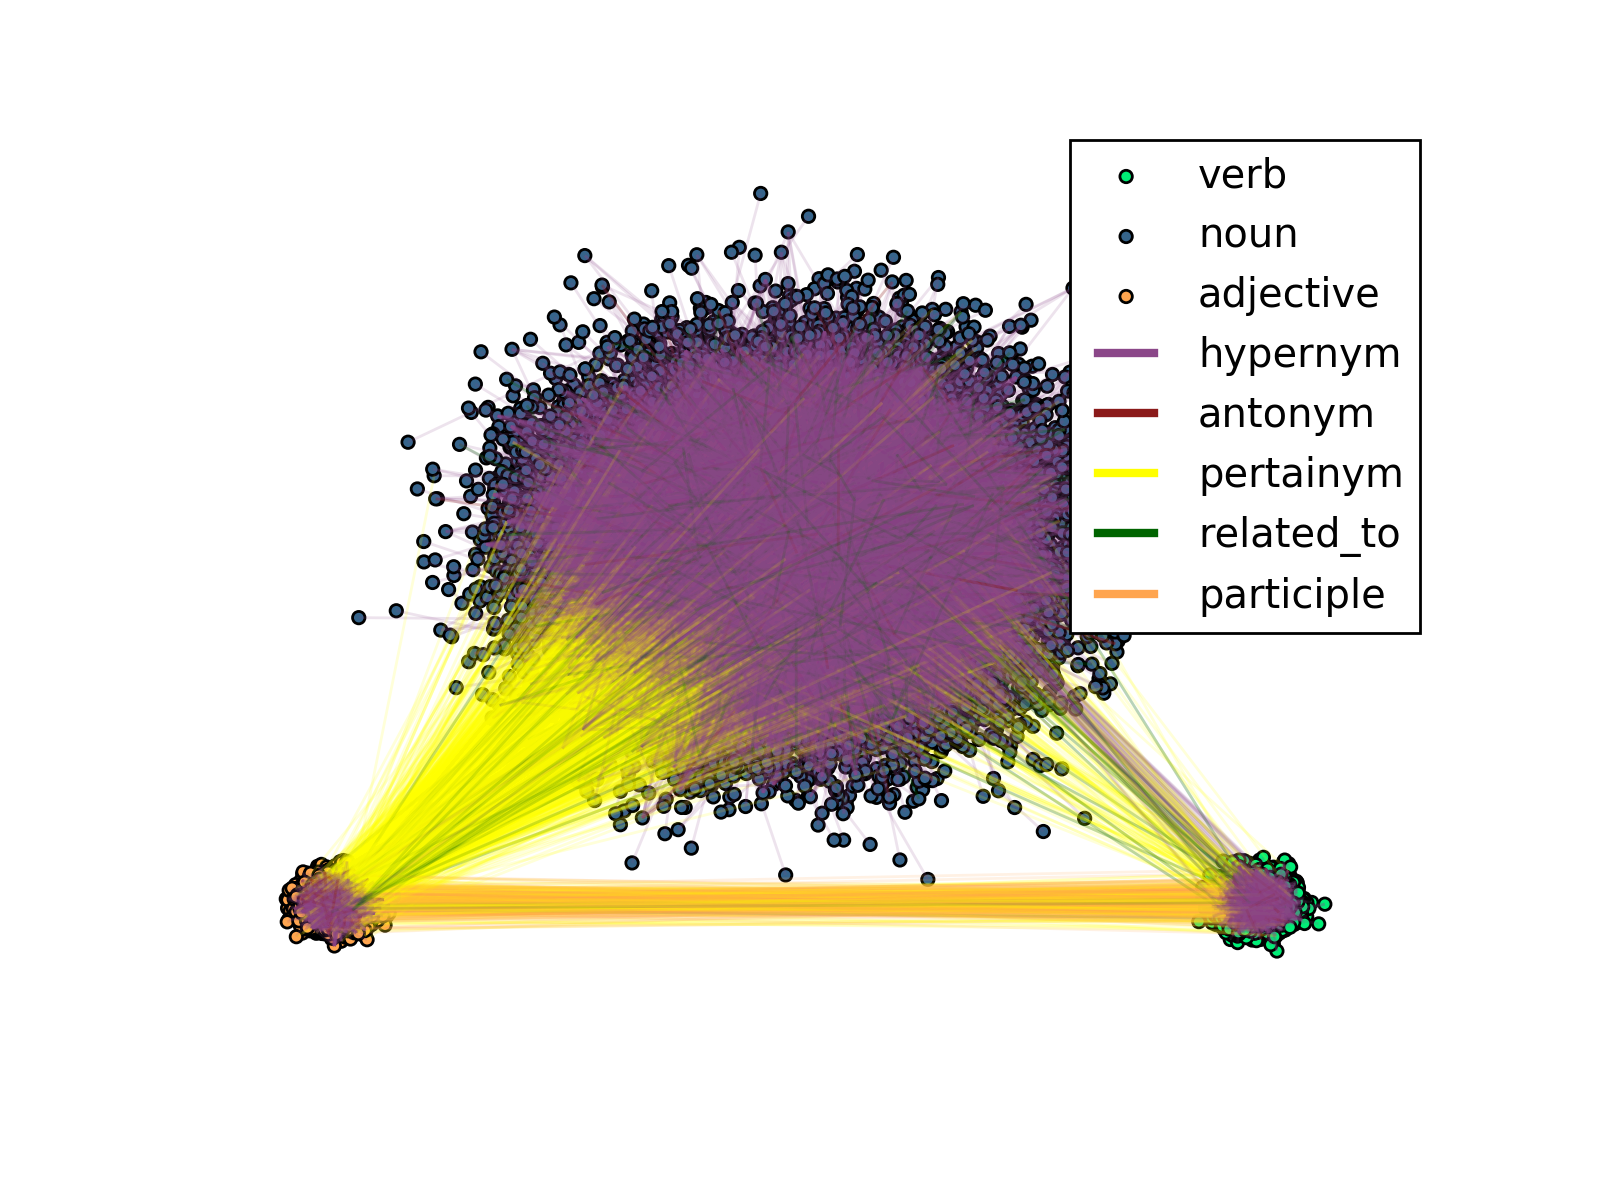
\includegraphics[width=\linewidth]{img/germanet.png}
  \caption{\textsc{GermaNet}}\label{snt-lex:fig:germanet}
\end{subfigure}%
\begin{subfigure}{.5\textwidth}
  \centering
  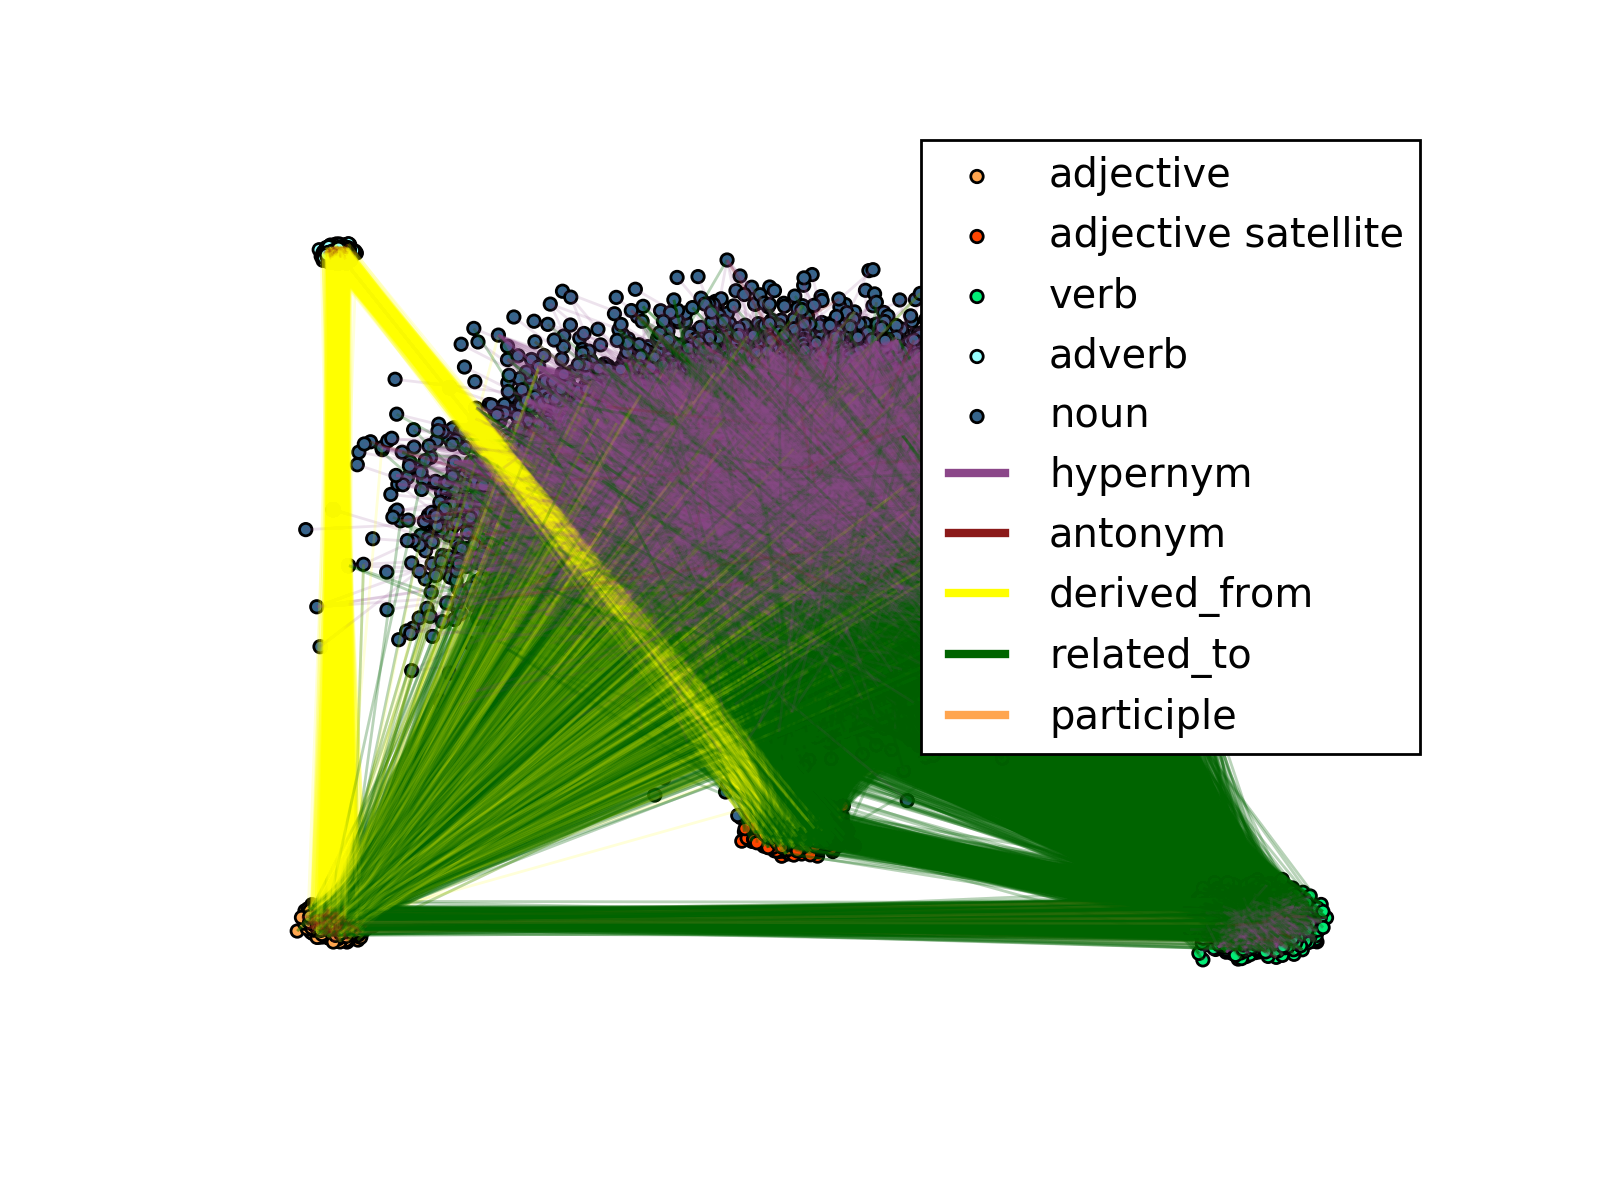
\includegraphics[width=\linewidth]{img/wordnet.png}
  \caption{\textsc{WordNet}}\label{snt-lex:fig:wordnet}
\end{subfigure}
}
\caption{Graphical visualization of \textsc{GermaNet} and
      \textsc{WordNet}.}\label{snt:fig:crp-sent-emo-distr}
\end{figure*}

As can be seen from the table, \textsc{GermaNet} has significantly
fewer words and synsets for all common parts of speech with the
largest gaps observed for nouns and adjectives.  Moreover, as shown in
Figures~\ref{snt-lex:fig:germanet} and~\ref{snt-lex:fig:wordnet}, such
PoS-classes as adverbs and adjective satellites are completely missing
in the German resource.  The reason for this is that the form (and
meaning) of most German adverbs typically coincides with that of the
adjectives; therefore, both categories are treated in the same way,
being represented through the adjectival synsets.

A slightly different situation can be observed for the semantic links
(relations) between the synsets: here, \textsc{GermaNet} features
almost 2,500 more hypernym-hyponym pairs than the English resource,
whereas the number of antonyms is more than four times less than in
\textsc{WordNet}.

An especially interesting pattern, however, appears with the relations
connecting different parts of speech: As can be seen from the figures,
the strongest inter-PoS connections in \textsc{GermaNet} are the
pertainym links between the adjectives and nouns and the participle
edges between the adjectives and verbs.  The interlinks between the
nouns and verbs, however, are both much fewer in number and more
diverse in their nature.  This situation is different in
\textsc{WordNet} where the prevailing majority of the
inter-part-of-speech connections are represented through the
\texttt{related\_to} (especially between the nouns, adjective
satellites, verbs, and verbs and adjectives) and
\texttt{derived\_from} links (especially between adverbs and
adjectives with their satellites).  The relations between the
adjectives and nouns are mixed though, featuring both
\texttt{related\_to} and \texttt{derived\_from} connections.  As we
should see later, these links are crucial for breaking part-of-speech
dependencies of seed sets in the cases when all seeds belong to the
same PoS class.

Another lexical sentiment resource (\textsc{WordNet-Affect}) was
proposed by \citet{Strapparava:04} who manually compiled a list of
1,903 subjective terms and projected these polarities to the
respective synononyms set in \textsc{WordNet}.  The resulting database
included 2,874 synsets with a total of 4,787 words.

% \subsubsection{Domain-Specific Sentiment Lexica}

% \citet{Chetviorkin:14} obtained a set of possible subjective terms
% from English and Russian microblogs by using an ensemble of supervised
% machine learning classifiers that had previously been trained on a
% manually annotated corpus of movie reviews.  In order to determine the
% prior polarity of the extracted terms, the authors first calculated
% approximate polarity scores of the processed messages using general
% polarity lexicons and then took these rough estimates as prior
% polarity expectations of the candidate expressions.  The posterior
% scores of these expressions were computed using the Ising spin model
% in a similar way to the approach proposed by \citet{Takamura:05}.  The
% resulting lexicon comprised 2,772 words for Russian and 2,786 lexical
% items for English.

\subsection{Summary and Conclusions}

In this section, we presented the first attempt of a practical
evaluation of our corpus.  In doing so, we addressed the task of
automatic prediction of polar terms (emotional expressions) with the
help of sentiment dictionaries.  To obtain a rough baseline estimate,
we first evaluated the quality of the existing sentiment lists for
German: German Polarity Clues~\cite{Waltinger:10},
SentiWS~\cite{Remus:10}, and Zurich Polarity List~\cite{Clematide:10}.
We showed that \ldots achieved the best quality, reaching an average
$F1$-score of \ldots on recognizing positive expressions and \ldots on
predicting negative polar terms.

In the next step, we analyzed whether the methods that were used for
creating the original English resources whose translations formed the
basis of the German lexica could yield better results than the
manually revised tranlated lists when applied to German data directly.

Another popular approach to an unsupervised induction of sentiment
lexica relies on the cooccurrence information about the words taken
directly from corpus.  One of the most popular methods from this
category is the Ising spin model adopted from the statistical
mechanics which interprets words as magnetic spins in a crystal grid
and tries to derive the most probable orientation of these spins in a
magnetic field.  This model was first applied to the needs of
computational linguistics by \citet{Takamura:05}, who induced a
sentiment lexicon for English using \ldots corpus data.  We have
reimplemented this approach in our program suite and applied to the
German Twitter snapshop of \citet{Scheffler:14}.  The results of this
approach are shown in Table~\ref{snt-lex:tbl:ispn-res}.

A different way of incorporating corpus data is to encode the
cooccurrence statistics directly into word information, representing
the latter as vectors.  We explored this direction in the final part
of this section, first obtaining word2vec embeddings for tokens from
the aforementioned snapshot and then applying clustering algorithms to
these representations.

Our results show that \ldots.

\newpage
